\chapter{Implementation, integration and testing plan}
This chapter presents the order of implementation of subsystems and components, 
the integration strategy and the testing plan.\\
Subsystems are developed and integrated using a bootm-up approach, starting from the 
individual parts and then linking them together.\\

\section{Implementation Plan}
The implementaton of the system is realised following a bottom-up method, with a particular 
emphasys on the back-end development since users will interact with the system only through 
its APIs.\\
Particularly, the implementation order is the following:
\begin{enumerate}
    \item \textbf{DBMS, DataManager:} this is the first part to be implemented since it is responsible 
    for storing and accessing the data needed by the system.
    \item \textbf{AuthManager:} this component is responsible for users authentication and authorization, 
    which are key aspects of the system, and therefore is heavily linked to the DBMS and DataManager.
    \item \textbf{MailManager, EvaluationTool:} these components can be implemented in parallel since they are 
    independent from each other.
    \item \textbf{CKBHandler:} this component is responsible for linking together the previous components, so 
    it must be developed after them.
    \item \textbf{UserApp:} this component is responsible for the interaction with the user, so it is to be 
    developed after the back-end have been completed.
\end{enumerate}
\section{Integration Plan}

\begin{figure}[H]
    \centering
    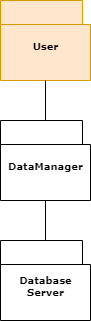
\includegraphics[width=0.2\textwidth]{images/integration_plan/first_level_integration.png}
    \caption{First level of integration}
\end{figure}

\begin{figure}[H]
    \centering
    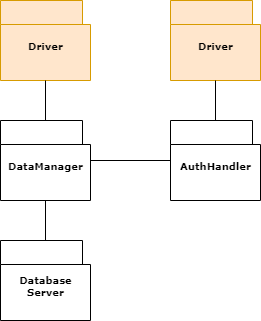
\includegraphics[width=0.45\textwidth]{images/integration_plan/second_level_integration.png}
    \caption{Second level of integration}
\end{figure}

\begin{figure}[H]
    \centering
    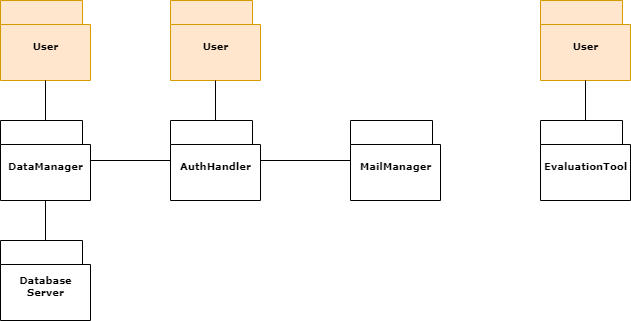
\includegraphics[width=1\textwidth]{images/integration_plan/third_level_integration.png}
    \caption{Third level of integration}
\end{figure}

\begin{figure}[H]
    \centering
    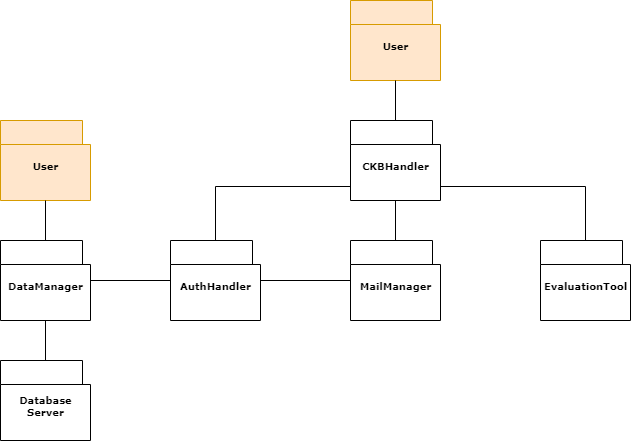
\includegraphics[width=1\textwidth]{images/integration_plan/fourth_level_integration.png}
    \caption{Fourth level of integration}
\end{figure}

\begin{figure}[H]
    \centering
    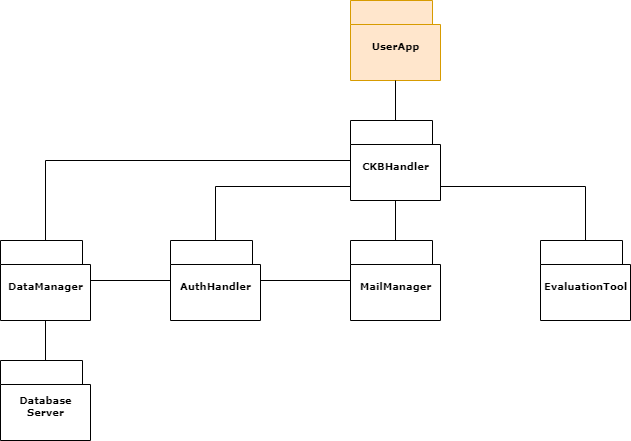
\includegraphics[width=1\textwidth]{images/integration_plan/fifth_level_integration.png}
    \caption{Fifth level of integration}
\end{figure}


\section{System Testing}
Testing should be performed both during and after the development of the system to ensure that all requirements 
are satisfied.\\
The testing plan is divided in two parts: unit testing and integration testing. Integration testing should also 
focus on the security aspects of the system to avoid any possible security breach.\\
Alpha testing should be performed whenever a new feature is implemented to receive feedback from the stakeholders 
regarding their level of satisfaction and eventual malfunctions.\\
A beta test phase could take place after the development of the system to ensure that the system is ready for 
a real-world usage and to collect information about performance and eventual scalability issues.\\